% Paquets généraux
\documentclass[a4paper,12pt,titlepage,twoside]{article}
\usepackage[T1]{fontenc}
\usepackage[utf8]{inputenc}
\usepackage[french]{babel}
\usepackage{subcaption}
\addto\captionsfrench{%
  \renewcommand{\tablename}{Tableau}%
}
\usepackage[gen]{eurosym}
%\usepackage[dvips]{graphicx}
\usepackage{minted}
\usepackage{fancyhdr}
\usepackage{pdfpages} 
\usepackage{multido}
\usepackage{hyperref}
\usepackage{textcomp}
\usepackage{schemabloc}
%\usepackage[bitstream-charter]{mathdesign}
\usepackage{array}
\newcolumntype{P}[1]{>{\centering\arraybackslash}p{#1}}
\usepackage[shortlabels]{enumitem}
\usepackage[framemethod=TikZ]{mdframed}

\newcommand{\id}{30}
\newcommand{\nom}{Calculs d'hyperstatisme}
\newcommand{\sequence}{04}
\newcommand{\nomsequence}{Liaisons entre les solides}
\newcommand{\num}{03}
\newcommand{\type}{TD}
\newcommand{\descrip}{En appliquant les règles de la théorie des mécanisme, déterminer le degré d'hyperstatisme de plusieurs systèmes et proposer des solutions afin de diminuer ce degré}
\newcommand{\competences}{B2-12: Proposer une modélisation des liaisons avec leurs caractéristiques géométriques. \\ &  B2-13: Proposer un modèle cinématique paramétré à partir d'un système réel, d'une maquette numérique ou d'u \\ &  B2-17: Simplifier un modèle de mécanisme. \\ &  B2-18: Modifier un modèle pour le rendre isostatique.}
\newcommand{\nbcomp}{4}
\newcommand{\systemes}{E.P.A.S, Machine d'essai de traction}
\newcommand{\systemesnum}{14, 13}
\newcommand{\systemessansaccent}{E.P.A.S, Machine d'essai de traction}
\newcommand{\ilot}{3}
\newcommand{\ilotstr}{03}
\newcommand{\dossierilot}{\detokenize{Ilot_03 E.P.A.S, Machine d'essai de traction}}
\newcommand{\imageun}{EPAS}
\newcommand{\imagedeux}{Machine_dessai_de_traction}

%\usepackage{style}
\usepackage{bodegraph}
\usepackage{rpcinematik}
\usepackage[locale = FR]{siunitx}
\usepackage{caption}
\newcommand{\institute}{Lycée Dorian}
\usepackage{calc}

\usepackage{listings}
\usepackage{fancyvrb}
\usepackage{color}
\usepackage{xcolor}
\usepackage{colortbl}
\usepackage{helvet}
\usepackage[frenchmath]{newtxsf} % for sans serif symbols
\renewcommand{\familydefault}{\sfdefault}
%\usepackage{amsfonts}
%\usepackage{amsmath}
%\usepackage{lmodern}
\usepackage{mathastext}
%\usepackage{xspace}
\usepackage{varioref}
\usepackage{tabularx}
%\usepackage{floatflt}
\usepackage{graphics}
\usepackage{wrapfig}
\usepackage{textcomp}
\usepackage{tikz,tkz-tab}
\usepackage[european resistor, european voltage, european current]{circuitikz}
\usepackage{wrapfig}
\usepackage{gensymb}
\usepackage[percent]{overpic}
\usetikzlibrary{babel}
\usepackage{ifthen}
\usepackage{cancel}
\usepackage{etoolbox}
\usepackage{multirow}
%\usepackage{boxedminipage}
\definecolor{gris25}{gray}{0.75}
\definecolor{bleu}{RGB}{18,33,98}
\definecolor{bleuf}{RGB}{42,94,171}
\definecolor{bleuc}{RGB}{231,239,247}
\definecolor{bleum}{RGB}{160,195,226}
\definecolor{rougef}{RGB}{185,18,27}
\definecolor{rougec}{RGB}{255,188,204}%255,230,231
\definecolor{vertf}{RGB}{103,126,82}
\definecolor{vertc}{RGB}{220,255,191}
\definecolor{forestgreen}{rgb}{0.13,0.54,0.13}
\definecolor{blcr}{rgb}{0.59,0.69,0.84}
\definecolor{blfr}{rgb}{0.32,0.51,0.75}
\definecolor{orfr}{rgb}{0.90,0.42,0.15}
\definecolor{orcr}{rgb}{0.90,0.65,0.50}
\definecolor{orangef}{rgb}{0.659,0.269,0.072}
\definecolor{orange}{rgb}{0.58,0.35,0.063}
\definecolor{orangec}{rgb}{0.43,0.32,0.25}
\definecolor{rcorrect}{rgb}{0.6,0,0}
\definecolor{sequence}{rgb}{0.75,0.75,0.75}
\definecolor{competences}{rgb}{0.61,0.73,0.35}
\definecolor{rose}{HTML}{ff00ff}
\definecolor{grisf}{HTML}{222222}
\definecolor{grisc}{HTML}{636363}
\definecolor{normal}{HTML}{4087c4}
\definecolor{info}{HTML}{5bc0de}
\definecolor{success}{RGB}{92,184,92}
\definecolor{warning}{RGB}{240,173,78}
\definecolor{danger}{RGB}{217,83,79}
\hypersetup{                    % parametrage des hyperliens
    colorlinks=true,                % colorise les liens
    breaklinks=true,                % permet les retours à la ligne pour les liens trop longs
    urlcolor= blfr,                 % couleur des hyperliens
    linkcolor= orange,                % couleur des liens internes aux documents (index, figures, tableaux, equations,...)
    citecolor= forestgreen                % couleur des liens vers les references bibliographiques
    }

\newcolumntype{M}[1]{>{\centering\arraybackslash}m{#1}}
\definecolor{codegreen}{rgb}{0,0.6,0}
\definecolor{codegray}{rgb}{0.5,0.5,0.5}
\definecolor{codepurple}{rgb}{0.58,0,0.82}
\definecolor{backcolour}{rgb}{0.95,0.95,0.92}

\lstdefinestyle{mystyle}{
    backgroundcolor=\color{backcolour},   
    commentstyle=\color{codegreen},
    keywordstyle=\color{magenta},
    numberstyle=\tiny\color{codegray},
    stringstyle=\color{codepurple},
    basicstyle=\ttfamily\footnotesize,
    breakatwhitespace=false,         
    breaklines=true,                 
    captionpos=b,                    
    keepspaces=true,                 
    numbers=left,                    
    numbersep=5pt,                  
    showspaces=false,                
    showstringspaces=false,
    showtabs=false,                  
    tabsize=2
}

\lstset{style=mystyle}

% Mise en page
\pagestyle{fancy}

\setlength{\hoffset}{-18pt}
\setlength{\oddsidemargin}{0pt} 	% Marge gauche sur pages impaire2s
\setlength{\evensidemargin}{0pt} 	% Marge gauche sur pages paires
\setlength{\marginparwidth}{00pt} 	% Largeur de note dans la marge
\setlength{\headwidth}{481pt} 	 	% Largeur de la zone de tête (17cm)
\setlength{\textwidth}{481pt} 	 	% Largeu\textbf{r de la zone de texte (17cm)
\setlength{\voffset}{-18pt} 		% Bon pour DOS
\setlength{\marginparsep}{7pt}	 	% Séparation de la marge
\setlength{\topmargin}{-30pt} 		% Pas de marge en haut
\setlength{\headheight}{55pt} 		% Haut de page
\setlength{\headsep}{20pt} 		% Entre le haut de page et le texte
\setlength{\footskip}{30pt} 		% Bas de\textbf{ page + séparation
\setlength{\textheight}{700pt} 		% Hauteur de l'icone zone de texte (25cm)
\setlength\fboxrule{1 pt}
\renewcommand{\baselinestretch}{1}
\setcounter{tocdepth}{1}
\newcommand{\cadre}[2]
{\fbox{
  \begin{minipage}{#1\linewidth}
   \begin{center}
    #2\\
   \end{center}
  \end{minipage}
 }
}

\newcommand{\repon}[1]
{
~\ \\
\begin{tabular}{|m{\linewidth}|}
 \hline
\multido{}{#1}{\\ \hline}
\end{tabular}
}


\newcommand{\objectif}[1]{
\mdfsetup{%
frametitle={%
\tikz[baseline=(current bounding box.east),outer sep=0pt]
\node[anchor=east,rectangle,fill=bleum]
{\strut Objectif~};}}
\mdfsetup{innertopmargin=10pt,linecolor=bleum,%
linewidth=2pt,topline=true,%
frametitleaboveskip=\dimexpr-\ht\strutbox\relax
}
\begin{mdframed}[]\relax%
#1
\end{mdframed}}


\newcounter{num_quest} \setcounter{num_quest}{0}
\newcounter{num_rep} \setcounter{num_rep}{0}
\newcounter{num_cor} \setcounter{num_cor}{0}

\newcommand{\feuilleDR}[1]{
	\begin{tikzpicture}
		\draw[gray!30](0,0)grid[step=0.5cm](\linewidth,#1);
	\end{tikzpicture}
}

%\newcommand{\question}[1]{\refstepcounter{num_quest}\par
%~\ \\ \parbox[t][][t]{0.15\linewidth}{\textbf{Question \arabic{num_quest}}}\parbox[t][][t]{0.85\linewidth}{#1\label{q\the\value{num_quest}}}\par
%}

\newcommand{\question}[1]{\refstepcounter{num_quest}\par
~\ \\ \textbf{Question \arabic{num_quest} : }#1\label{q\the\value{num_quest}}\par
}

\newcommand{\posetafigure}[3]{
\begin{figure}[ht!]
 \begin{center}
  \includegraphics[width=#2\linewidth]{img/#1}
 \end{center}
 \caption{\label{#1} #3}
\end{figure}}

\newcommand{\goforum}{
\begin{figure}

\end{figure}
\begin{center}
 \includegraphics[width=0.7\linewidth]{../../../img/go_forum}
\end{center}
\label{go_forum}
\caption{J'pète les plombs}
\end{figure}}

\newcommand{\reponse}[4][1]
{\noindent
\parbox{\textwidth}{
\rule{\linewidth}{.5pt}\\
\textbf{Question\ifthenelse{#1>1}{s}{} \multido{}{#1}{%
\refstepcounter{num_rep}\ref{q\the\value{num_rep}} }:} ~\ \\
\ifdef{\public}{#3 \ifthenelse{#2>0}{~\ \\ 	\feuilleDR{#2}}}{#4}
}}

\newboolean{printdr}
\newboolean{printcor}
\setboolean{printdr}{false}
\setboolean{printcor}{false}

\newcommand{\reponseinfo}[2][1]
{\noindent
\rule{\linewidth}{.5pt}\\
\textbf{Question\ifthenelse{#1>1}{s}{} \multido{}{#1}{%
\refstepcounter{num_rep}\ref{q\the\value{num_rep}} }:} ~\ \\
\ifdef{\public}{\parbox{\textwidth}{\ifthenelse{#2>0}{~\ \\ 	\feuilleDR{#2}}}
\setboolean{printdr}{true}\setboolean{printcor}{false}}
{\setboolean{printdr}{false}\setboolean{printcor}{true}}
}

\makeatletter
\newcommand\modulo[2]{
    \newcounter{lastpagesujet}
	\setcounter{lastpagesujet}{#1}
    \divide\value{lastpagesujet} by #2
    \multiply\value{lastpagesujet} by #2
    \advance\value{lastpagesujet} by #2
    \advance\value{lastpagesujet} by 1\relax
    }
\makeatother

\newcommand{\finsujet}[1]
{
    \begin{center}
    \Large{FIN}
    \end{center}
        
    \ifthenelse{\equal{#1}{public}}{\def\public{}}{}

	\newpage

}

\newcommand{\debutcor}
{	
    \ifdef{\public}{
    	\modulo{\value{page}-1}{4}
		\whiledo{\value{page}<\value{lastpagesujet}}{~\ \newpage}
        \pagestyle{docreponse}
	}{\pagestyle{correction}}

    \ifdef{\public}{
        \begin{tikzpicture} 
            \draw (0,0) rectangle (2,2);
            \draw (0,0) -- (2,2);
            \draw (1.5,0.5) node {\large 20};
            \draw (2.5,0) rectangle (16,2);
            \draw (4.5,1.7) node {\large Commentaires:};
        \end{tikzpicture}
    }
    ~\ \\
}

%\newcommand{\repcarre}[2]
%{
%~\ \\
%\begin{tikzpicture}
%\draw [fill=white] (0,0) rectangle +(\linewidth,#1);
%\node[align=left] at (1.1,#2-0.3) {\textbf{Question #1:}};
%\end{tikzpicture}
%}

\newcommand{\titre}[1]
{\begin{center}
\cadre{0.8}{\huge #1} 
\end{center}
}


%Définition des torseurs :
\newcommand{\torseur}[2]{\left\{\mathcal{#1}_{#2} \right\}}
\newcommand{\torseurh}[3]{\left\{\genfrac{}{}{0pt}{0}{#1}{#2}\right\}_{#3}}
\newcommand{\torseurv}[8]{\left\{
\begin{matrix}
#1 & #4 \\ #2 & #5 \\ #3 &#6
\end{matrix}
\right\}_{{#7},{#8}}}

%Définition des torseurs :
%\newcommand{\torseur}[2]{\left \{\mbox{\relsize{2}{$\mathcal {#1}$}\relsize{-2}}\phantom{}_{\mbox{\scriptsize $#2$}} \right \}}
%\newcommand{\torseurh}[3]{\left\{\genfrac{}{}{0pt}{0}{#1}{#2}\right\}_{#3}}
%\newcommand{\torseurv}[8]{
%\left\{\begin{array}{@{}c|c@{}} #1 & #4 \\ #2 & #5 \\ #3 & #6 \end{array} \right\}_{#7,#8}
%}
\newcommand{\derivee}[2]{\left.\dfrac{\d #1}{\d t}\right|_{#2}}
\newcommand{\tripleint}{\int\!\!\!\!\!\int\!\!\!\!\!\int}

% Notation cinématique et statique
\newcommand{\cinematique}[2]{\mbox{#1}/\mbox{#2}}
\newcommand{\statique}[2]{\mbox{#1}\rightarrow\mbox{#2}}
\newcommand{\moment}[3]{\vv {#1}_{\scriptsize{#3}}(#2)}
\newcommand{\resultante}[2]{\vv {#1}_{\scriptsize{#2}}}


%Commande de base
\newcommand{\jo}{\left(j\omega\right)} % j \omega dans l'analyse fréquentielle
\newcommand{\tl}{\xrightarrow{\mathcal{L}}} % transformée de laplace sur fleche
\newcommand{\tli}{\xrightarrow{\mathcal{L}^{-1}}} % transformée inverse de laplace sur fleche
\renewcommand{\d}[1][]{\mathrm{d#1}}
\newcommand{\dd}[1][]{\mathrm{d#1}}
\newcommand{\vect}[2]{{#1}\wedge{#2}}
\newcommand{\base}[3]{(\vec #1,\vec #2,\vec #3)}
\newcommand{\vectbase}[4]{{\vphantom{\left| \begin{matrix}
#1\\#2\\#3 \end{matrix} \right|}}_{#4}{\left| \begin{matrix}
#1\\#2\\#3 \end{matrix} \right.}}
%Pour avoir les paragraphes sous la forme I, II, III
\renewcommand{\thesection}{\Roman{section}}
\setcounter{secnumdepth}{3}
\renewcommand{\Frlabelitemii}{$\bullet$}

% En tête et pied de page
\lhead{\nom}
\rhead{\includegraphics[width=2cm]{../../../img/logo}}
\lfoot{\auteurun,\ \auteurdeux}
\cfoot{Page \thepage}

\fancypagestyle{docreponse}{%
  \fancyhf{}
  \fancyhead[LO]{NOM Prénom: .............................}
  \rhead{\includegraphics[width=2cm]{../../../img/logo}\hspace{2pt}}
  \ifdef{\auteurdeux}{\lfoot{\auteurun,\ \auteurdeux}}{\lfoot{\auteurun}}
  \rfoot{\nom}
  \lfoot{Document réponse}
  \cfoot{Page \thepage}
   }

\fancypagestyle{correction}{%
  \fancyhf{}
  \lhead{\colorbox{danger}{\begin{minipage}{0.65\paperwidth} \textcolor{white}{\textbf{Correction}} \end{minipage}} }
  \rhead{\includegraphics[width=2cm]{../../../img/logo}}
  \lfoot{Renaud Costadoat, Françoise Puig}
  \rfoot{\colorbox{danger}{\begin{minipage}{0.3\paperwidth} \begin{flushright}\textcolor{white}{\textbf{Correction}}\end{flushright} \end{minipage}} }
  \cfoot{Page \thepage}
}

\fancypagestyle{correctioninfo}{%
  \fancyhf{}
  \lhead{\colorbox{danger}{\begin{minipage}{0.65\paperwidth} \textcolor{white}{\textbf{Correction}} \end{minipage}} }
  \rhead{\includegraphics[width=2cm]{../../../img/logo}}
  \lfoot{Renaud Costadoat, Juliette Genzmer}
  \rfoot{\colorbox{danger}{\begin{minipage}{0.6\paperwidth} \begin{flushright}\textcolor{white}{\textbf{Correction}}\end{flushright} \end{minipage}} }}

\renewcommand{\footrulewidth}{0.4pt}

\usepackage{eso-pic}
\newcommand{\BackgroundPic}{%
\put(0,0){%
\parbox[b][\paperheight]{\paperwidth}{%
\vfill
\begin{center}
\hspace{0.5cm}\vspace{0.5cm}
\includegraphics[width=\paperwidth,height=\paperheight,%
keepaspectratio]{../../../img/fond3}%
\end{center}
\vfill
}}}

\newcommand{\BackgroundPicdeux}{%
\put(25,-30){%
\parbox[b][\paperheight]{\paperwidth}{%
\vfill
\begin{center}
\includegraphics[width=\paperwidth,height=\paperheight,%
keepaspectratio]{../../../img/fond4}%
\end{center}
\vfill
}}}

\begin{document}

\pagestyle{empty}

\AddToShipoutPicture*{\BackgroundPic}

\includegraphics[width=2cm]{../../../img/logo}

\Huge{DS \numero - \sujet}

\vspace{1cm}

\ifdef{\prive}{\begin{center}\colorbox{danger}{\Huge{Avec Correction}}\end{center}}{}

\begin{center}
\centering\huge{PTSI}
\end{center}

\vspace{2cm}


\begin{center}
\centering\Large{\jour}
\end{center}

\vspace{2cm}

\normalsize

\tableofcontents

\newpage

\AddToShipoutPicture{\BackgroundPicdeux}

\pagestyle{fancy}

\begin{center}
\Huge \sujet
\end{center}


\normalsize


\section{Présentation du système}

\subsection{Contexte}

Ce concept a été inventé au Canada en 2008, et s'est étendu à toute l'Amérique du Nord avant de traverser l'Atlantique pour proposer un cinéma dynamique avec une quantité d'effets spéciaux et spatiaux. Le fauteuil dynamique de cinéma est principalement destiné à l'industrie du divertissement et de la simulation.

Pour ressentir au mieux ces sensations, la technologie permet désormais de ressentir dans son fauteuil les différents mouvements, par de fortes vibrations et accélérations. Ce système repose sur la post-synchronisation des films. Comme pour un doublage ou un sous-titrage, les mouvements du film sont transmis au fauteuil.

Si la plate-forme à six degrés de liberté s'est imposée dans le cas des simulateurs de vols, elle ne répond pas aux exigences plus étendues des fauteuils dynamiques. Des solutions spécifiques à un environnement de simulation aussi réaliste que possible nécessitent le recours à un système de restitution des mouvements. Le système étudié est une évolution en cours d'étude des fauteuils dynamiques actuellement commercialisés, qui s'inspire des sièges dynamiques utilisés pour l'entrainement des pilotes d'avion de chasse (voir figure \ref{fig1}).

\begin{figure}[!ht]
\begin{minipage}{0.35\linewidth}
 \centering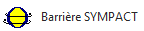
\includegraphics[width=0.8\linewidth]{img/img01}
\end{minipage}\hfill
\begin{minipage}{0.55\linewidth}
 \centering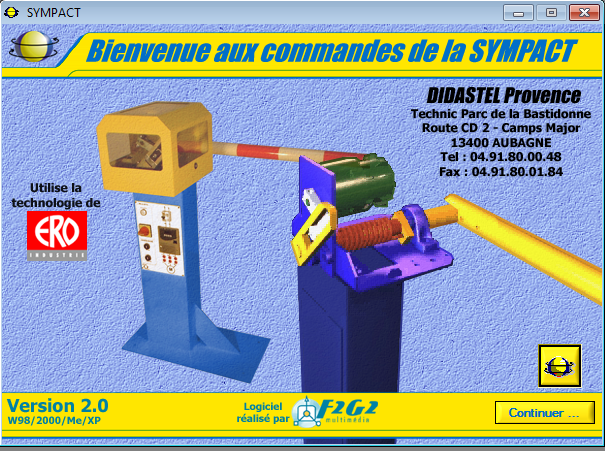
\includegraphics[width=1\linewidth]{img/img02}
\end{minipage}

\begin{center}
 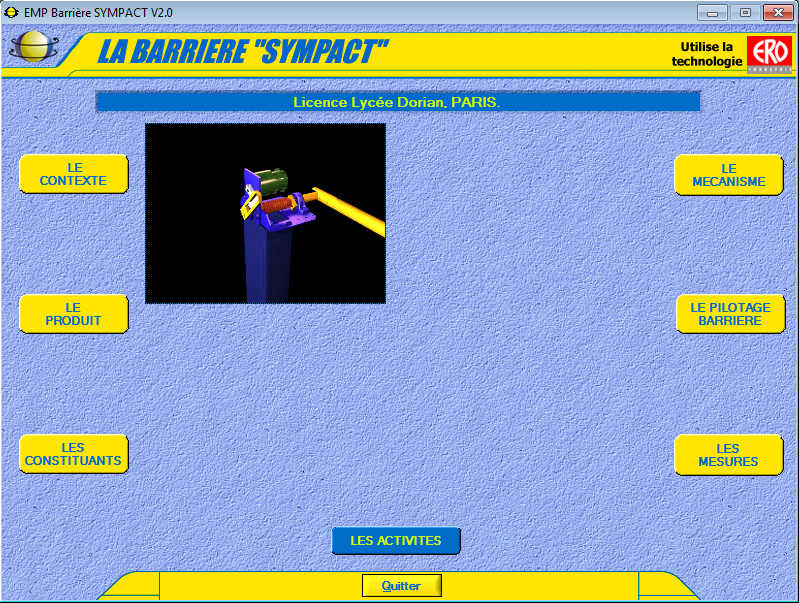
\includegraphics[width=0.8\linewidth]{img/img03}
\end{center}
\caption{Modèles de sièges}
\label{fig1}
\end{figure}


\subsection{Mise en situation}

Le siège dynamique est constitué :
\begin{itemize}
 \item du dosseret (voir figure \ref{fig2}) qui permet d'agir directement sur la tête du spectateur afin d'amplifier la sensation d'accélération (via l'oreille interne). Le point de contact entre le dosseret et la tête du spectateur est matérialisé par le point D,
 \item de l'assise du siège (voir figure \ref{fig3}) qui permet d'obtenir un mouvement de tangage et un mouvement de roulis du spectateur.
\end{itemize}

\begin{figure}[!ht]
\begin{center}
 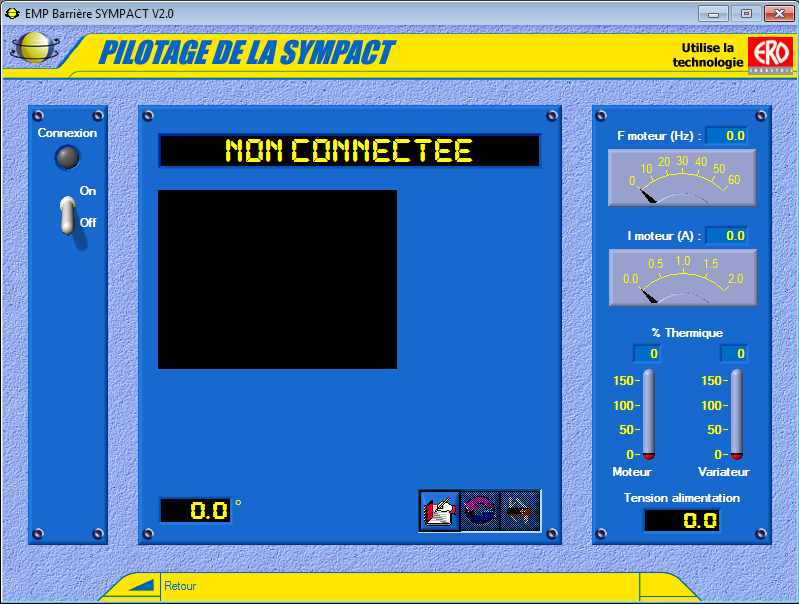
\includegraphics[width=0.8\linewidth]{img/img04}
\end{center}
\caption{Dosseret}
\label{fig2}
\end{figure}

\begin{figure}[!ht]
\begin{center}
 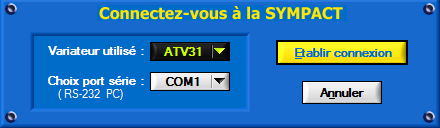
\includegraphics[width=0.8\linewidth]{img/img05}
\end{center}
\caption{Assise du siège}
\label{fig3}
\end{figure}

Les trois motorisations (une pour le dosseret et deux pour l'assise) sont composées chacune d'un moteur à courant continu à aimants permanents et d'un réducteur de vitesse. Chaque moteur est alimenté par un variateur de vitesse dont la structure de puissance est un hacheur. Un capteur de courant interne au variateur est utilisé par ce accouplée à l'axe de chaque moteur est utilisée par le variateur correspondant pour réaliser un asservissement de vitesse. Un codeur incrémental accouplé aussi sur l'axe de chaque moteur est utilisé par une carte à base de microcontrôleur pour réaliser un asservissement de position, une sortie analogique de cette carte étant reliée à l'entrée de consigne du variateur de vitesse.

\subsection{Étude proposée}

Les accélérations procurées aux spectateurs sont un élément fondamental qui conditionne la conception et la réalisation de ce fauteuil dynamique de cinéma. Les solutions technologiques retenues répondent à cet objectif. Elles ne sont pas toutes abordées dans ce sujet. Quelques unes de celles retenues pour le fauteuil dynamique de cinéma sont étudiées pour valider les solutions choisies par les concepteurs vis-à-vis des performances attendues listées par le cahier des charges. Dans cette optique, il est proposé au candidat les trois études suivantes :
\begin{itemize}
 \item modélisation, validation et optimisation de certains constituants associés à l'exigence fonctionnelle \og amplifier la sensation d'accélération \fg,
 \item validation de l'architecture de la chaine fonctionnelle réalisant l'exigence fonctionnelle \og incliner le spectateur suivant l'axe de tangage et de roulis \fg,
 \item synthèse globale de l'étude proposée.
\end{itemize}

\section{Exigence fonctionnelle \og amplifier la sensation d'accélération \fg}

\textbf{Objectif}

Proposer un modèle de comportement des éléments réalisant l'exigence fonctionnelle \og amplifier la sensation d'accélération »\fg puis valider les performances attendues listées par le cahier des charges (figure \ref{fig4}).

\begin{figure}[!ht]
\begin{tabular}{|p{2cm}|p{8cm}|p{5cm}|}
\hline
\textbf{Exigence} & \textbf{Critères d'appréciation} & \textbf{Niveau} \\
\hline
\multirow{3}{2cm}{Amplifier la sensation d'accélération} & Précision statique de la boucle d'asservissement de position:
\begin{itemize}
 \item Erreur statique de position,
 \item Erreur statique de trainage,
 \item Erreur statique d'accélération.
\end{itemize}
& \par ~\ \par ~\ \par <1\% \par <1\% \par <1\% \par \\
\cline{2-3}
& Rapidité pour un échelon de consigne d'accélération:
\begin{itemize}
 \item Temps de montée de 0 à 100\% de la consigne 
 \item Dépassement	
\end{itemize}
& \par ~\ \par ~\ \par ~\ \par <5ms \par <20\% \\
\cline{2-3}
& Accélération maximale du point D de la tête du spectateur situé à 85 mm au-dessus de l'axe de rotation du dosseret & $6m.s^{-2} < a_{max} < 7m.s^{-2}$ \\
\hline
\end{tabular}
\caption{Extrait du cahier des charges associé à l'exigence fonctionnelle \og Amplifier la sensation d'accélération \fg réalisée par le dosseret}
\label{fig4}
\end{figure}

\newpage

\subsection{Notations et hypothèses}

Le schéma multi physique modélisant l'asservissement de position du dosseret est fourni (figure \ref{fig5}).
Le schéma-bloc retenu pour la modélisation de l'asservissement de position du dosseret est fourni (figure \ref{fig6}).

\begin{tabular}{|p{2cm}|p{7cm}|p{2cm}|p{2cm}|}
\hline
 & \textbf{Description} & \textbf{Variable temporelle} & \textbf{Unité} \\
\hline
$\theta_{Cd}(p)$ & consigne de position du dosseret	& $\theta_{Cd}(t)$ & rad \\
\hline
$\theta_{C}(p)$ & consigne de position de l'axe moteur & $\theta_{C}(t)$ & rad \\
\hline
$\theta(p)$ & position de l'axe moteur & $\theta(t)$ & rad \\
\hline
$\theta_{r}(p)$ & position de l'axe de sortie du réducteur & $\theta_{r}(t)$ & rad \\
\hline
$\theta_{d}(p)$ & position du dosseret & $\theta_{d}(t)$ & rad \\
\hline
$N_{Codeur}(p)$ & valeur numérique issue du comptage incrémental & $N_{Codeur}(t)$ & 	 \\
\hline
$r$ & rapport de transmission du réducteur & &  \\
\hline
$K_{c}$ & gain du mécanisme  de la transformation de mouvement du dosseret & &  \\
\hline
\end{tabular}

\begin{figure}[!ht]
\begin{center}
 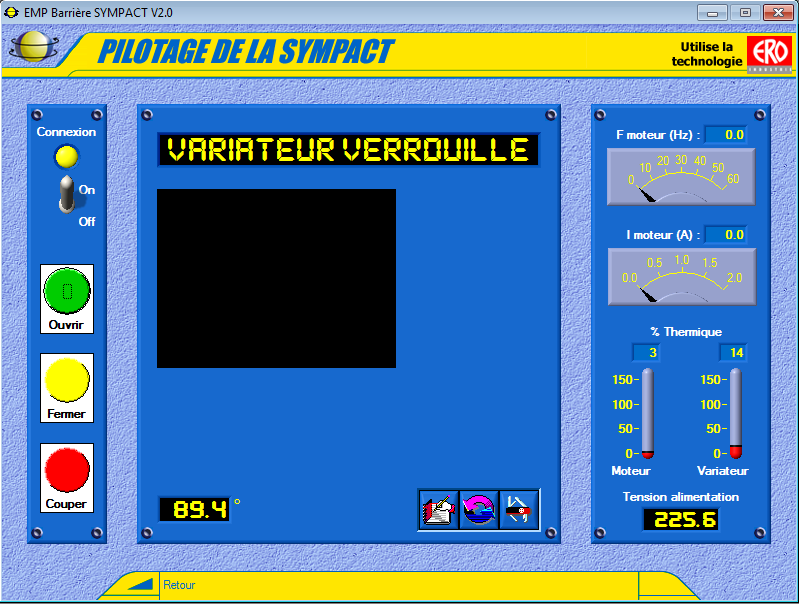
\includegraphics[width=\linewidth]{img/img06}
\end{center}
\caption{Schéma multi-physique  de l'asservissement du dosseret}
\label{fig5}
\end{figure}

\begin{figure}[!ht]
\begin{center}
 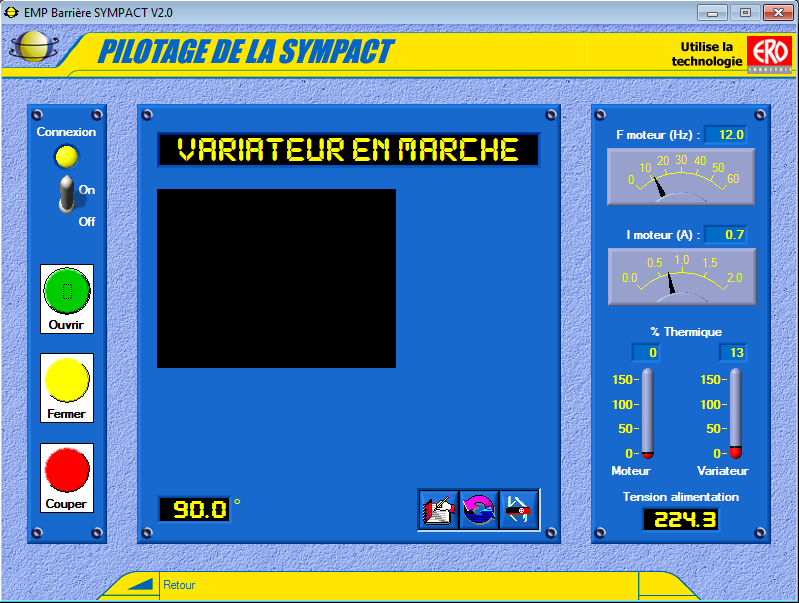
\includegraphics[width=\linewidth]{img/img07}
\end{center}
\caption{Schéma-bloc de l'asservissement du dosseret}
\label{fig6}
\end{figure}

\clearpage

\begin{tabular}{|p{2cm}|p{7cm}|p{2cm}|p{2cm}|}
\hline
 & \textbf{Description} & \textbf{Variable temporelle} & \textbf{Unité} \\ \hline
$c$ & gain du codeur incrémental & & $rad^{-1}$ \\ \hline
$a$ & gain proportionnel du correcteur de l'asservissement de position & & $V$ \\ \hline
$U_{C\Omega}(p)$ & image de la consigne de vitesse de l'axe moteur & $u_{C\Omega}(t)$ & $V$ \\ \hline
$\Omega(p)$ & vitesse de l'axe moteur & $\Omega(t)$ & $rad.s^{-1}$ \\ \hline
$C_{\Omega}(p)$ & correcteur de l'asservissement de vitesse	& &  \\ \hline
$I_C(p)$ & image de la consigne de courant & $i_C(t)$	& $V$ \\ \hline
$C_I(p)$ & correcteur de l'asservissement de courant & & \\ \hline
$h$ & gain du hacheur & & \\ \hline
$K_{rI}$ & gain du capteur de courant & &  \\ \hline
$U(p)$ & tension d'alimentation du moteur & $u(t)$ & $V$ \\ \hline
$E(p)$ & force électromotrice du moteur	& $e(t)$ & $V$ \\ \hline
$I(p)$ & courant dans l'induit  du moteur & $i(t)$ & $A$ \\ \hline
$C_M(p)$ & couple moteur & $c_M(t)$ & $N.m$ \\ \hline
$C_R(p)$ & couple résistant perturbateur & $c_R(t)$ & $N.m$ \\ \hline
$L$ & inductance du circuit d'induit du moteur & & \\ \hline
$R$ & résistance du circuit d'induit du moteur & & \\ \hline
$K_{\Omega}$ & gain de la génératrice tachymétrique	& & $V.s.rad^{-1}$ \\ \hline
$K$ & gain de la constante de couple ou de la constante de force électromotrice	& &  \\ \hline
$J$ & moment d'inertie  de l'ensemble  en mouvement, ramené  au  niveau  de l'axe moteur & &  \\ \hline
$f$ & coefficient de frottements visqueux équivalent pour l'ensemble en mouvement & &  \\ \hline
\end{tabular}

Données: \\
\begin{itemize}
 \item $K = 0,115 N.m.A^{-1}(V.s.rad^{-1})$
 \item $R = 1 \Omega$
 \item $L = 1,1mH$
 \item $K_{rI}= 0,5 V. A^{-1}$
 \item $h = 6$
 \item $r = 1/50$
 \item $f = 4.10^{-4} N.m.s.rad^{-1}$
 \item $J=0,16.10^{-3} kg.m^2$
 \item Correcteur de courant $C_I(p)=k_2.(1+\dfrac{1}{T_2.p})$, avec $k_2 = 5$ et $T_2=0,3ms$,
 \item Correcteur de vitesse $C_{\Omega}(p)=k_1.(1+\dfrac{1}{T_1.p})$, avec $k_1=20$
\end{itemize}

Hypothèses: \\
\begin{itemize}
 \item La période d'échantillonnage est suffisamment faible pour être négligeable devant la dynamique globale du système et les différentes variables sont donc toutes considérées comme des fonctions continues du temps,
 \item Le temps de réponse du hacheur est considéré négligeable dans l'étude,
 \item Les conditions de Heaviside sont vérifiées.
\end{itemize}

\subsection{Comportement cinématique du mécanisme de transformation de mouvement du dosseret}

\textbf{Objectif:}\\
Valider la linéarité du comportement du mécanisme de transformation de mouvement du dosseret (figure \ref{fig7}) en établissant la loi de comportement cinématique.

Le modèle cinématique de la transformation de mouvement du dosseret est fourni figure \ref{fig8}.

\paragraph{Question 1:} À l'aide d'une fermeture géométrique, exprimer littéralement l'angle $\theta_d$ en fonction de l'angle $\theta_r$. Mettre l'expression sous la forme :
\begin{center}
$cos\theta_d.(E+F.cos\theta_r)+sin\theta_d.(G+F.sin\theta_r)=H+(I.cos\theta_r+J.sin\theta_r)$
\end{center}

Une simulation numérique a permis d'obtenir le tracé représenté sur la figure \ref{fig9}. Afin d'obtenir un modèle linéaire de la caractéristique $\theta_d=f(\theta_r)$, l'étude se fait autour de son point de fonctionnement statique pour de petites variations.

\paragraph{Question 2:} Déterminer par linéarisation autour du point de fonctionnement $\theta_r=0\text{°}$, la valeur numérique du gain dynamique $K_C$ de la transformation de mouvement du dosseret.

\begin{figure}[!ht]
\begin{center}
 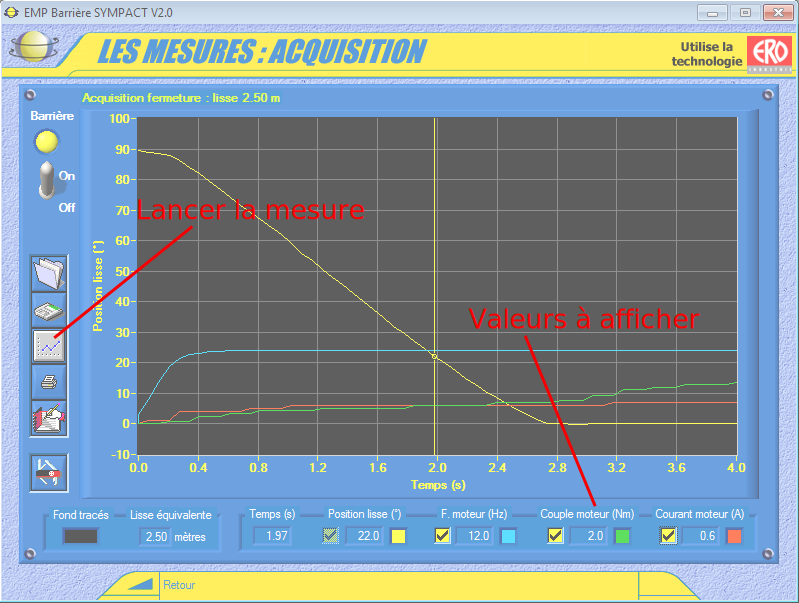
\includegraphics[width=0.9\linewidth]{img/img08}
\end{center}
\caption{Mécanisme de transformation de mouvement du dosseret}
\label{fig7}
\end{figure}

\subsection{Comportement du codeur incrémental et de la génératrice tachymétrique}

\textbf{Objectif:}\\
Établir un modèle de comportement du codeur incrémental et de la génératrice tachymétrique.
Le moteur AXEM a pour référence F12M4. Il est alimenté par une carte variateur de vitesse RTS 10-20-60 (PARVEX) alimentée sous $60V DC$ et pouvant délivrer $20A$ pendant $2s$, avec un courant nominal de $10A$.

Ce dernier comprend les boucles d'asservissement de vitesse et de courant. Sur l'arbre moteur sont montés une génératrice tachymétrique et un codeur incrémental $250 points.tour^{-1}$. Le comptage incrémental est effectué sur le front montant d'une des deux voies. La génératrice tachymétrique est raccordée à l'entrée de retour vitesse du variateur. Un réglage par potentiomètre présent dans le variateur est effectué pour obtenir une tension de $5V$ au niveau du comparateur de l'asservissement de vitesse lorsque la fréquence de rotation du moteur est égale à $3000tr.min^{-1}$.

\paragraph{Question 3:} En tenant compte des informations précédentes, calculer la valeur numérique de $c$ et de $K_{\Omega}$ (figure \ref{fig6}).

\textit{Commentaire: Vous ferez attention aux unités données dans le tableau \ref{fig4}.}

\subsection{Comportement de l'ensemble variateur et moteur du dosseret}

\textbf{Objectif:}\\
Valider un modèle simplifié de l'asservissement de position de l'axe moteur afin d'analyser les paramètres influant sur la précision et proposer une amélioration du système.

Pour cela, il faut :
\begin{itemize}
 \item établir un modèle simplifié de l'asservissement de courant,
 \item établir un modèle simplifié de l'asservissement de vitesse,
 \item analyser la précision de l'asservissement de position.
\end{itemize}

\subsubsection{Modélisation de l'asservissement du courant}

L'étude suivante consiste à vérifier la validité de la simplification du modèle de la boucle d'asservissement du courant de la figure \ref{fig10} par le modèle de la figure \ref{fig11}.

Pour le modèle de la figure \ref{fig10} lorsque $C_R(p)=0$, la fonction de transfert s'écrit :

\begin{center}
$\dfrac{\Omega(p)}{I_C(p)}=\dfrac{Kk_2hT_2p+Kk_2h}{T_2LJp^3+(T_2(Lf+RJ)+k_2hk_{rI}T_2 J)p^2+(T_2(Rf+K^2)+k_2hk_{rI}(T_2f+J))p+k_2hk_{rI}f}$
\end{center}

À l'aide d'un logiciel de simulation, une comparaison du comportement de la vitesse en sortie des deux modèles a été effectuée (figure \ref{fig12}) et ce pour un échelon unitaire de consigne de courant appliqué en entrée.

\newpage

\begin{figure}[!ht]
\begin{center}
 \includegraphics[width=0.7\linewidth]{img/img09}
\end{center}
\caption{Modèle cinématique de la transformation de mouvement du dosseret}
\label{fig8}
\end{figure}

\begin{figure}[!ht]
\begin{center}
 \includegraphics[width=0.7\linewidth]{img/img10}
\end{center}
\caption{Représentation de l'équation de fermeture géométrique}
\label{fig9}
\end{figure}

\paragraph{Question 4:}	Pour chacun des deux modèles (initial et simplifié), quelle est la valeur finale de $\Omega(t)$ lorsque $i_c(t)$ est un échelon unitaire ? À l'aide de ces résultats et des relevés issus de la simulation dans le régime transitoire, conclure quant à la validité de la simplification du modèle sachant que chaque sollicitation du dosseret a une durée d'environ $30 ms$.

\textit{Commentaire: Attention, on ne demande que la valeur finale}

\begin{figure}[!ht]
\begin{center}
 \includegraphics[width=0.9\linewidth]{img/img11}
\end{center}
\caption{Modèle initial de la boucle d'asservissement de courant}
\label{fig10}
\end{figure}

\begin{figure}[!ht]
\begin{center}
 \includegraphics[width=0.6\linewidth]{img/img12}
\end{center}
\caption{Modèle simplifié de la boucle d'asservissement de courant}
\label{fig11}
\end{figure}

\begin{figure}[!ht]
\begin{center}
 \includegraphics[width=0.9\linewidth]{img/img13}
\end{center}
\caption{Tracés}
\label{fig12}
\end{figure}

\subsubsection{Modélisation de l'asservissement de vitesse}

L'étude suivante consiste à obtenir un modèle simplifié de la boucle d'asservissement de vitesse (figure \ref{fig13}) au regard des réglages effectués et de l'influence d'une perturbation de type échelon sur le dosseret. En effet, vu la courte durée des sollicitations, la perturbation sur le dosseret, dont l'origine peut être une action du spectateur sur ses muscles cervicaux, peut être modélisée par un échelon.

\begin{figure}[!ht]
\begin{center}
 \includegraphics[width=0.9\linewidth]{img/img14}
\end{center}
\caption{Modèle de la boucle d'asservissement de vitesse}
\label{fig13}
\end{figure}

\paragraph{Question 5:}	Exprimer la fonction de transfert de la boucle de vitesse $H_{\Omega}(p)=\dfrac{\Omega(p)}{U_{C\Omega}(p)}$, lorsque $C_R(p)=0$. Rappel : $C_{\Omega}(p)=k_1.(1+\dfrac{1}{T_1. p})$

\paragraph{Question 6:}	$T_1$ étant égal à $\dfrac{J}{f}$, montrer alors que la fonction de transfert en boucle fermée peut se mettre sous la forme $\dfrac{b}{\tau.p+1}$. Calculer les valeurs numériques des termes $b$ et $\tau$.

\paragraph{Question 7:} En déduire, à l'aide de la figure \ref{fig13}, $\dfrac{\theta(p)}{C_R(p)}$ lorsque $\theta_C(p)=0$. Calculer ensuite la valeur finale de $\theta(t)$ lorsque $c_R(t)$ est un échelon unitaire. Conclure quant à l'action, en régime permanent, du correcteur proportionnel et intégral sur les effets d'une perturbation $c_R(t)$ de type échelon.

\textit{Commentaire: Il faudra pour cela déplacer le sommateur de $C_R(p)$, si vous avez oublié la méthode il est possible de la retrouver en transformant un extrait du schéma bloc en équation.}

\subsubsection{Modélisation de la boucle d'asservissement de position}

Après toutes les simplifications précédentes, est obtenu le modèle de la figure \ref{fig14} où seul le comportement en réponse à la consigne $\theta_C$ est abordé.

\begin{figure}[!ht]
\begin{center}
 \includegraphics[width=0.7\linewidth]{img/img15}
\end{center}
\caption{Modèle simplifié de la boucle d'asservissement de position}
\label{fig14}
\end{figure}

\paragraph{Question 8:} Exprimer la fonction de transfert $\dfrac{\theta(p)}{\theta_C(p)}$. Déterminer ensuite la valeur numérique de $a$ pour avoir un facteur d'amortissement égal à 0,7. Justifier le choix de ce facteur d'amortissement. (Pour ce calcul et les calculs suivants prendre $b=63rad.s^{-1}.V^{-1}$, $\tau=2,2ms$, $c=40rad^{-1}$.)

\subsubsection{Analyse de la précision du système}

Un aspect important pour la simulation sensorielle du siège dynamique est la capacité du système à reproduire fidèlement la consigne de position issue du programme de simulation sensorielle du siège dynamique. Dans un premier temps, l'étude se limite à la précision statique en utilisant le modèle défini à la figure \ref{fig14}. L'erreur représente la différence entre l'entrée $\theta_C(t)$ et la sortie $\theta(t)$ et est définie par la variable $\mu(t)=\theta_C(t)-\theta(t)$.

La précision statique du système est définie par les trois paramètres suivants :
\begin{itemize}
 \item $\mu_p=\lim\limits_{t \rightarrow +\infty} \mu(t)$, suite à une entrée de type échelon unité ($\theta_C(t)=u(t)$,$\theta_C(p)=\dfrac{1}{p}$) appelé erreur de position,
 \item $\mu_v=\lim\limits_{t \rightarrow +\infty} \mu(t)$, suite à une entrée de type rampe ($\theta_C(t)=t.u(t)$,$\theta_C(p)=\dfrac{1}{p^2}$) appelé erreur de trainage ;
 \item $\mu_a=\lim\limits_{t \rightarrow +\infty} \mu(t)$,suite à une entrée de type accélération ($\theta_C(t)=\dfrac{t^2.u(t)}{2}$,$\theta_C(p)=\dfrac{1}{p^3}$) appelé erreur en accélération.
\end{itemize}

\paragraph{Question 9:} Exprimer dans un premier temps $\mu(p)$ en fonction de $\theta_C(p)$, puis déterminer de façon littérale et numérique l'erreur de position $\mu_p$, l'erreur de trainage $\mu_v$ et l'erreur en accélération $\mu_a$. Conclure quant à la précision statique du système suite aux différentes consignes $\theta_C(p)$ de type échelon, rampe et accélération.

\subsection{Validation de la performance simulée en accélération du dosseret}

\textbf{Objectif:}\\
Valider la performance simulée en accélération au regard du cahier des charges fonctionnel.

Grâce à la modélisation de la chaine fonctionnelle réalisée précédemment, un logiciel de simulation permet d'obtenir la courbe de la vitesse angulaire maximale $\dot{\theta}_d$ (figure \ref{fig15}) ainsi que celle de l'accélération angulaire maximale $\ddot{\theta}_d$ (figure \ref{fig15}) du dosseret. Ces deux courbes sont tracées sur une durée de $30ms$ lors du démarrage du moteur (au-delà de ce temps le moteur atteint sa vitesse nominale).

\begin{figure}[!ht]
\begin{center}
 \includegraphics[width=0.9\linewidth]{img/img16}
\end{center}
\caption{Vitesse et accélération angulaires en fonction du temps}
\label{fig15}
\end{figure}

\paragraph{Question 10:} Déterminer, à partir du paramétrage donné figure \ref{fig8}, l'expression littérale au point D (représentant le point de contact avec la tête du spectateur) du vecteur accélération $\overrightarrow{\Gamma}_{D\in dosseret/chassis}$. Calculer numériquement la norme de ce vecteur accélération au point D correspondant à la valeur maximale de $\ddot{\theta}_d$.

\paragraph{Question 11:} Conclure quant au respect du nombre de $g$ du cahier des charges (figure \ref{fig4}) vis-à-vis des accélérations simulées produites par le dosseret du siège dynamique de cinéma.

\subsubsection{Optimisation des performances du dosseret}

La figure \ref{fig16} représente la structure d'une correction par anticipation qui permet d'améliorer la précision statique du système

\begin{figure}[!ht]
\begin{center}
 \includegraphics[width=0.8\linewidth]{img/img17}
\end{center}
\caption{Structure avec anticipation}
\label{fig16}
\end{figure}

\paragraph{Question 12:} Déterminer l'erreur de position $\mu_p$ puis l'erreur de trainage $\mu_v$. Conclure sur l'erreur de position au regard du cahier des charges.

\paragraph{Question 13:} D'après l'erreur de trainage $\mu_v$ déterminée à la question précédente, calculer la valeur numérique de $d$ qui permet d'annuler cette erreur de trainage. En prenant en compte la valeur numérique de $d$ et de $b$, déterminer l'expression de l'erreur en accélération $\mu_a$. Calculer ensuite sa valeur numérique et conclure au regard du cahier des charges.

Un aspect important pour la simulation sensorielle du siège dynamique est la capacité du système à reproduire rapidement les consignes d'accélération. À l'aide d'une simulation, la variable accélération $\ddot{\theta}_d$ possède les deux comportements donnés figure \ref{fig17} pour la période transitoire, et ce lorsque la consigne vaut $\theta_{Cd}(t)=\dfrac{t^2}{2}.u(t)$.

\newpage 

\begin{figure}[!ht]
\begin{center}
 \includegraphics[width=0.8\linewidth]{img/img18}
\end{center}
\caption{Accélération du dosseret avec et sans anticipation}
\label{fig17}
\end{figure}

\paragraph{Question 14:} Conclure quant au respect du cahier des charges vis-à-vis des accélérations produites par le dosseret du siège dynamique de cinéma.

\section{Conception du montage d'une roue de charriot}

\subsection{Fabrication de l'arbre}

Des spécifications ont été mises en place sur le mécanisme afin de garantir le bon fonctionnement du système.

\paragraph{Question 15:} Donner la signification des spécifications suivantes en complétant les tableaux GPS donnés en document réponse.
\\ ~\ \\
\begin{minipage}{0.45\linewidth}
\centering\includegraphics[width=2.5cm]{img/specif1}
\end{minipage}\hfill
\begin{minipage}{0.45\linewidth}
\centering\includegraphics[width=2.5cm]{img/specif2}
\end{minipage} ~\ \\

\subsection{Fabrication du chapeau}

Le chapeau suivant permet de bloquer les roulements à bille. ~\ \\

\begin{center}
 \includegraphics[width=5cm]{img/specif3}
\end{center}\hfill

\paragraph{Question 16:} Comment est réalisée la mise en position du chapeau sur le système ? (centrage court, centrage long, nature des surfaces: point, droite, plan, cercle, cone, sphère,...)

\paragraph{Question 17:} Proposer une solution de spécification des surfaces indiquées \og Surfaces à spécifier \fg à partir des références. Cette spécification doit être réalisée sur le document réponse.

\subsection{Montage de roulements}
 
Le montage d'une roue de charriot est à concevoir dans la suite. Le montage à mettre en place est un montage en X.

Contraintes:\\
\begin{itemize}
 \item Le serrage axial doit être réglable,
 \item Le système doit être démontable,
 \item Des roulements à rouleaux doivent être utilisés.
\end{itemize}

\paragraph{Question 18:} Compléter les zones 1a et 1b, en intégrant les deux roulements à mettre en place.

Dans la zone 1a, le roulement est placé entre les pièces 9 et 2, il faut prévoir une étanchéité dynamique de ce côté, pour empêcher le lubrifiant présent à l'intérieur de la pièce 2 de s'échapper par la gauche.

Dans la zone 1b, le roulement est placé entre les pièces 9 et 6, la fermeture par un chapeau permet de conserver le lubrifiant à l'intérieur de la pièce 2 de ce côté.

Vous mettrez en place les ajustements nécessaires au montage.

\subsection{Fixation de la roue}

La fixation de la roue s'effectue par la mise en place d'un écrou à encoches.

\paragraph{Question 19:} Mettre en place l'écrou et la rondelle à encoches dans la zone 2 du dessin.

\includepdf[page=20,scale=0.9,angle=90]{Ressource/Sujet_BTS.pdf}

\clearpage ~\ \clearpage 

\includepdf[scale=0.9,angle=90]{img/doc_rep2.pdf}

\includepdf[scale=0.9,angle=90]{img/doc_rep2.pdf}

\includepdf[scale=0.9,angle=90]{img/doc_rep3.pdf}

\ifdef{\public}{\end{document}}{}

\newpage
\cleardoublepage

\pagestyle{correction}\setcounter{section}{0}

\section{Correction}


\end{document}

